%   ____ _                 _              _____ 
%  / ___| |__   __ _ _ __ | |_ ___ _ __  |___ / 
% | |   | '_ \ / _` | '_ \| __/ _ \ '__|   |_ \ 
% | |___| | | | (_| | |_) | ||  __/ |     ___) |
%  \____|_| |_|\__,_| .__/ \__\___|_|    |____/ 
%%%%%%%%%%%%%%%%%%%%%%%%%%%%%%%%%%%%%%%%
\chapter{SELECTED TEST CASES AND IMPLEMENTATIONS}
\label{ch_cases}
%%%%%%%%%%%%%%%%%%%%%%%%%%%%%%%%%%%%%%%%

In this chapter, each one of the test cases is defined by an algorithm and a specific application, followed by the corresponding implementations in F90 and the chosen Python HPC implementations. The three selected test cases are:   

\begin{itemize}

\item\autoref {sec_stencil}: Stencil test case, applied to a heat transfer problem on a finite 2D surface solved by a finite-difference method.

\item\autoref {sec_fft}: FFT test case, applied to a 3D array of synthetic data.

\item\autoref {sec_forest}: The Random Forest test case, applied to a classification problem of asteroid orbits.

\end{itemize}

Please refer to \autoref {sec_sdenviron} for the description of the different processing nodes of the Santos Dumont supercomputer. 

In all implementations of the different test cases, the open-source web application JupyterLab was used to experiment, develop, execute and analyze the results, including the F90 implementations. It allows the sharing of codes, data, and documents that were used to manage these implementations and allows interactive code-related functions to be implemented and executed interactively, and to check the reproducibility of the results.

%
%
%
%
%
%
%
%  ____  _                  _ _ 
% / ___|| |_ ___ _ __   ___(_) |
% \___ \| __/ _ \ '_ \ / __| | |
%  ___) | ||  __/ | | | (__| | |
% |____/ \__\___|_| |_|\___|_|_|
%----------------------------------------
\section{Stencil test case and implementations}
\label{sec_stencil}
%----------------------------------------

Processing performances of the Python implementations were evaluated, taking as references the serial and parallel F90 corresponding implementations. The adopted test case is a well known heat transfer problem over a finite surface (\autoref {fig_calor1e2}), modeled by the Poisson partial-differential equation. It models the normalized temperature distribution over the surface along a number of iterations that compose the simulation. As commonly employed for numerical solutions, this equation is discretized in a finite grid and solved by a finite difference method. 

    \begin{figure}[hbtp]
    \caption{Initial and final temperature distribution over a finite surface exemplified for a $10 \times 10$  blue-cell grid, including constant zero-temperature boundary conditions in the outer borders, and thus the simulation encompasses only the $8 \times 8$ inner grid. Three heat sources were arbitrarily chosen, shown as \fcred{red} cells.}
    \vspace{4mm}
    \begin{minipage}[t]{.46\textwidth}
    \begin{center}
    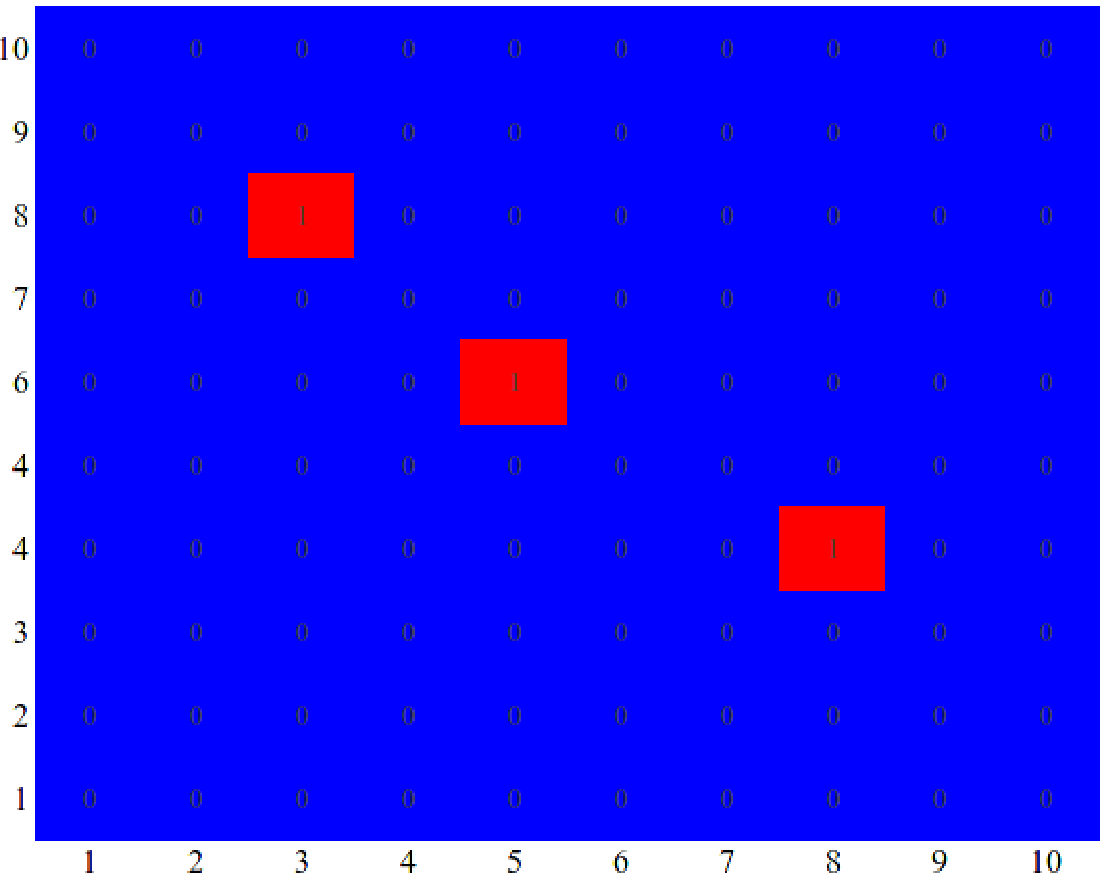
\includegraphics[width=.9\linewidth]{fig_calor1}
    \end{center}
    \vspace{3mm}
    \legenda{(a) Initial zero-temperature distribution over the $10 \times 10$ grid for a finite surface. }
    \end{minipage}
    \hfill
    \begin{minipage}[t]{.46\textwidth}
    \begin{center}
    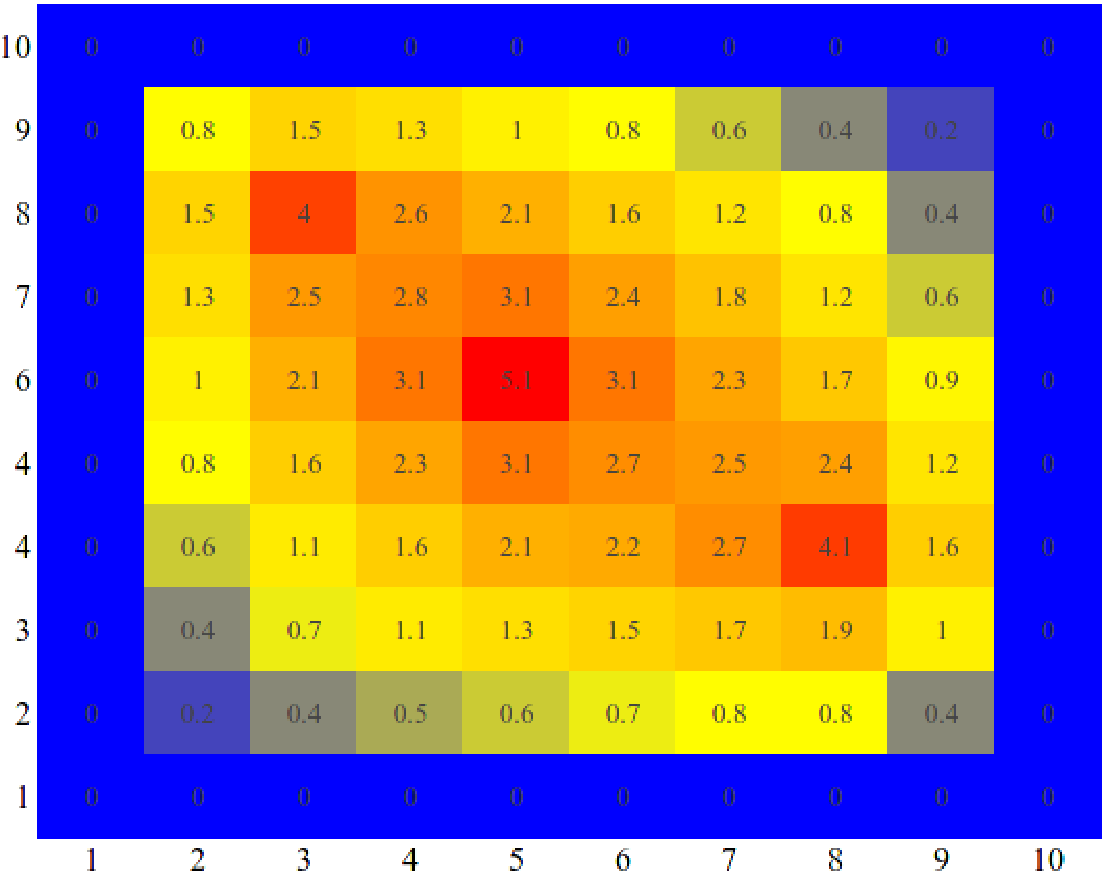
\includegraphics[width=.91\linewidth]{fig_calor2}
    \end{center}
    \vspace{3mm}
    \legenda{(b) Final temperature distribution for the same grid after 500 iterations.}
    \end{minipage}
    \vspace{5mm}
    \legenda{}
    \FONTE{Author's production.}
    \label{fig_calor1e2}
    \end{figure}

The specific algorithm is based on a main loop for time steps. In each iteration (time step), the 2D grid is updated and the temperature of the 3 grid points of the heat sources is increased by 1 unit, modeling the insertion of energy that is performed every time step. The updating of the 2D grid requires the calculation of a five-point stencil over the 2D domain grid \cite {Chen2002} in order to update the temperatures at every time step. A uniform temperature field with zero value is assumed over the surface, and typically, adiabatic or Dirichlet  boundary conditions are assumed, being the latter assumed for this problem. Three constant rate heat sources were placed at localized grid points, and each introduces a unit amount of heat at each time step. The heat transfer simulation is modeled over a finite number of time steps, with all grid points being updated at each time step. The temperature distribution will be determined by the heat sources and the Dirichlet boundary conditions, which implies in zero temperature at the border grid points. 

The five-point stencil allows updating a grid point by averaging the temperatures of the point itself with the temperatures of its four neighboring grid points, left-right and up-down. The temperature field $U$ is defined over a discrete grid $(x,y)$ with spatial resolutions  $\Delta x = \Delta y = h$. Thus, the discretization maps real Cartesian coordinates $(x,y)$ to a discrete grid $(i,j)$, with $U_{x,y}=U_{i,j} \, , \,  U_{x+h,y}=U_{i+1,j} \,$ for the $x$ dimension, and analogously for the $y$ dimension. Therefore, the discretized 2D Poisson equation with a five-point stencil is expressed by \autoref {eq_poisson}.

\begin{equation}
  \frac{\partial^2 U}{\partial x^2} +
  \frac{\partial^2 U}{\partial y^2} \approx
  \frac{U_{i+1,j}+U_{i,j+1}-4U_{i,j}+U_{i-1,j}+U_{i,j-1}}{h^2}
  \label{eq_poisson}
\end{equation}

In the case of parallelization, the domain corresponding to the finite surface is divided into subdomains that are assigned to processes or threads. However, the update of points in the border of subdomains requires the temperatures values of points in the neighboring subdomains, and such data dependency between subdomains implies in communication between processes or synchronization between threads \cite {Langtangen2008a}. Considering the chosen test case, an early implementation of the algorithm was proposed by \citeonline {Balaji2017} using the C language, but later it was ported to F90. \autoref {fig_calor1e2}(b) shows the final temperature distribution over a finite surface after 500 iterations, exemplified by the grid 10 × 10 and three arbitrarily chosen heat sources, shown as \fcred{red} cells. The simulation covers only the internal grid 8 × 8, and the initial zero-temperature distribution is indicated in blue.

The 2D discrete domain is shown in \autoref {fig_malh}(a), with every small circle denotes a grid point and the \fcred{red} cross, the five-point stencil. \fcgreen{Green} lines show the division of the domain into 9 equal subdomains, for the sake of example. The same domain is shown in \autoref {fig_malh}(b), but with each subdomain enlarged by two rows and two columns of extra grid points, shown in yellow, which are copies of the grid points of the four neighboring subdomain. In the borders of the domain, grid points corresponding to the boundary conditions are copied. These extra rows and columns of grid points compose the ghost zone of each subdomain for the specific five-point stencil, with other stencils eventually requiring a different number of rows and columns of grid points. The \fcred{red} arrow denotes the communication/synchronization required to update a grid point of the central subdomain from a ``white point'' of the subdomain above it, with the temperature of this point copied to the corresponding ``yellow point'' of the ghost zone of the considered central subdomain.

    \begin{figure}[hbtp]
    \caption{Discretized 2D domain of the heat transfer case (red cross denotes the five-point stencil).}
    %\vspace{2mm}
    \begin{minipage}[t]{.46\textwidth}
    \begin{center}
    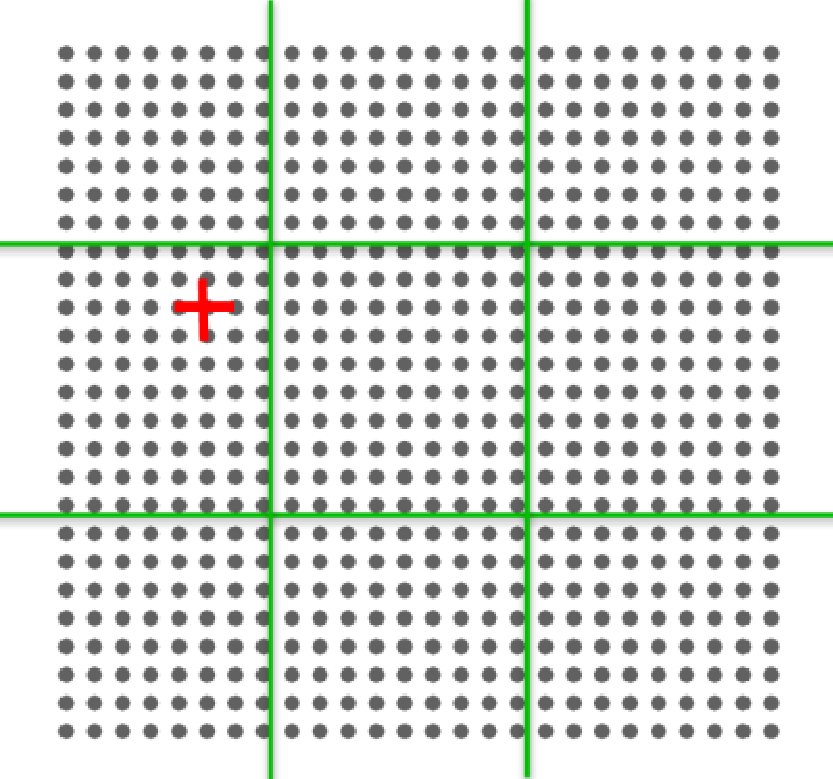
\includegraphics[width=.65\linewidth]{fig_malhdivi}
    \end{center}
    \vspace{3mm}
    \legenda{(a) Discretized 2D domain of the heat transfer problem chosen as test case showing 9 sub domains with their grid points.}
    \end{minipage}
    \hfill
    \begin{minipage}[t]{.46\textwidth}
    \begin{center}
    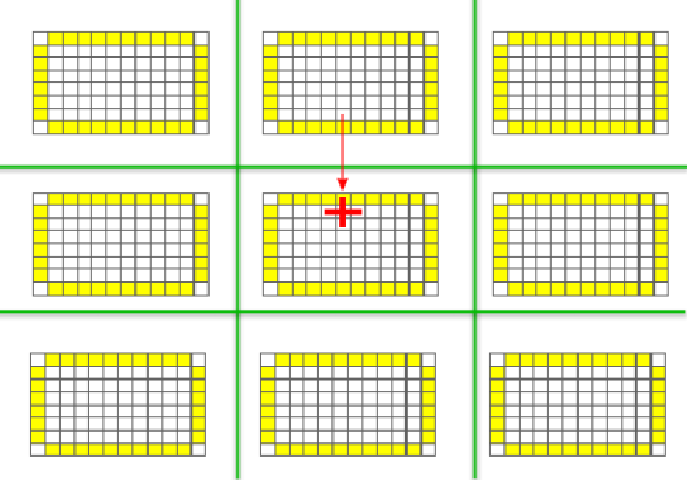
\includegraphics[width=\linewidth]{fig_malhtran}
    \end{center}
    \vspace{3mm}
    \legenda{(b) Discretized 2D domain of the heat transfer problem divided into 9 sub domains enlarged with their ghost zones.}
    \end{minipage}
    \vspace{6mm}
    \legenda{}
    \FONTE{Adapted from \citeonline {Balaji2017}.}
    \label{fig_malh}
    \end{figure}

For simplification, it is assumed a square grid of $n \times n = N$ points, and also a square grid of processors or threads of $p \times p = P$ units, in a way that $n$ is a multiple of $p$. It is then possible to divide the domain into $P$ subdomains, each one containing $[ N/P = (n \times n) / (p \times p) = n/p \times n/p ]$ points. The ghost zone then adds two rows and two columns of grid points, considering the five-point stencil.  Therefore, each subdomain contains $ [ (n+2)/p \times (n+2)/p ] $ points.

Serial and parallel of the Stencil test case F90 implementations were based on a former work \cite {Renato2018}. Other implementations are standard Python, Fortran-to-Python (F2PY), Cython, and Numba (including Numba-GPU). The compute-intensive part of the implementations was hand coded and does not use an existing off-the-shelf external library. In this work, most parallel versions of these implementations are based on MPI: the version is wrapped by the MPI for Python (mpi4py) API into a Python function, allowing the execution of MPI processes in one or more computing nodes from the Python environment. However, the F2PY API is the only exception, since it reuses a binary code generated by an F90 compiler by encapsulating it into a Python function. Parallelization using threads was restricted to the execution of a Numba JIT-compiled function in GPU, which is also discussed ahead.

Stencil test case implementations are described in the next sections.

%
%
%
%----------------------------------------
\subsection{F90 serial and parallel} % Stencil
\label{sec_stenimplf90}
%----------------------------------------

The F90 serial and parallel versions were compiled with the GNU-compiler gfortran, which fully complies to the Fortran 95 standard. The serial F90 version is the implementation of the algorithm described in the previous section. Its corresponding parallel version employs standard MPI asynchronous non-blocking communication functions \textit {MPI\_ISend()} and \textit {MPI\_IRecv()}, which allows overlapping computation and communication, enhancing the parallel performance. However, at the end of each time step, synchronization is required for the updating of each subdomain ghost zones from the neighboring subdomains. As already mentioned, for a square grid with $N = n \times n $ points and $p \times p$ MPI processes, each process is assigned a subdomain with a total of $[(N/p)+2] \times [(N/p)+2]$ points, including the ghost zone. The compute-intensive  part of the code is the updating of the domain grid using the five-point stencil, as shown in the F90 code of the \autoref {lst_stf90}, showing two nested loops that traverse the 2D grid, with the \textit {anew} array stores the values of updated grid elements calculated from their previous values \textit {aold} array.

\begin{lstlisting}[float=hbt, language=Fortran, label={lst_stf90}, caption={Compute-intensive part of the Stencil test case F90 code.}]
do j = 2, by+1
    do i = 2, bx+1
        anew(i,j) = ( aold(i, j) / 2.0 +
                    ( aold(i-1,j) + aold(i+1,j) +
                      aold(i,j-1) + aold(i,j+1) ) / 8.0 )
    enddo
enddo
\end{lstlisting}

%
%
%
%----------------------------------------
\subsection{F2PY serial and parallel} % Stencil
\label{sec_stenimplf2py}
%----------------------------------------

F2PY creates a Python library from the F90/C code, and this library is then imported by the Python code. In this test case, the function arguments of the created library are the number of grid points, the location and heat rate of the sources, the number of iterations, etc. If the F90 code is not already parallelized with MPI, a typical alternative is to use the mpi4py Python library in the Python code. F2PY seems to be convenient when an optimized F90/C code already exists and can be reused. In this test case, the Python code uses F90/C code wrapped into a library built by F2PY, as shown in the \autoref {lst_stf2p}. The Pyhton library libstencil is built by F2PY from F90 code, and includes the function funcstencil. The parameters \textit {gridsize}, \textit {energy}, \textit {niters}, are the same as in the F90 implementation, and the total energy entered into the grid and the elapsed time are returned by the function and stored in the variables \textit {heat} and \textit {etime}.

\begin{lstlisting}[float=hbt, language=Python, label={lst_stf2p}, caption={Compute-intensive part of the F2PY implementation, in the main Python code.}]
heat, etime = libstencil.funcstencil(gridsize, energy, niters)
\end{lstlisting}

%
%
%
%----------------------------------------
\subsection{Standard Python serial and parallel} % Stencil
\label{sec_stenimplpy}
%----------------------------------------

The portability of the F90 code to Python is straightforward, requiring only NumPy as external library, which is the Python numerical-tool library. Most of the loops in the Python code can be executed using NumPy. The structure and sequence of the original code is preserved and executed interactively by the Python interpreter, while the cycle of analyzing results, changing code or parameters, and re-executing, benefits from the JupyterLab environment. However, as any interpreted language, Python is slow. Once the proof-of-concept of the Python code is complete, the code needs to be optimized, focusing on its compute-intensive parts, which are the performance bottlenecks. In this step, the programmer can take advantage of the modular nature of Python to selectively optimize the code, for example by porting a specific module to F90 or by replacing it by an optimized library function. In addition, parallelization can be performed employing the native Python multiprocessing environment. In this work, Python multiprocessing was provided by the MPI for Python (mpi4py) library. The compute-intensive part of the code is the updating of the domain grid using the five-point stencil at each timestep, as shown in the Python code in the \autoref {lst_sfpyt}. Two nested loops traverse the 2D grid, and the \textit {anew} array stores the result of an equation that uses the elements of the \textit {aold} array. Loops are performed internally by NumPy using the colon notation (``:'') in the array indices.

\begin{lstlisting}[float=hbt, language=Python, label={lst_sfpyt}, caption={Compute-intensive part of the Python implementation.}]
anew[1:-1,1:-1] = ( aold[1:-1,1:-1] / 2.0 +
                  ( aold[2:,1:-1] + aold[:-2,1:-1] +
                    aold[1:-1,2:]  + aold[1:-1,:-2] ) / 8.0 )
\end{lstlisting}

%
%
%
%----------------------------------------
\subsection{Cython serial and parallel} % Stencil
\label{sec_stenimplcy}
%----------------------------------------

Cython is a compiler for both the Cython and Python languages, which is typically used to create Python libraries. These libraries are later called from standard Python code. In this test case the original Python code was reused, with few changes, in order to be compiled by Cython. The Cython parallel version employs mpi4py. The part that updates the 2D grid using the five-point stencil is shown in the \autoref {lst_stcyt}.

\begin{lstlisting}[float=hbt, language=Python, label=lst_stcyt, caption={Compute-intensive part of the Cython implementation.}]
cpdef stp(double[:,::1] anew, double[:,::1] aold, Py_ssize_t by, Py_ssize_t bx):
    for i in range(1, bx+1):
        for j in range(1, by+1):
            anew[i,j] = ( aold[i,j] / 2.0 +
                        ( aold[i-1,j] + aold[i+1,j] +
                          aold[i,j-1] + aold[i,j+1] ) / 8.0 )
\end{lstlisting}

In this Cython implementation, the code included comments starting with ``\#cython:'' that are actually compiler directives for disabling limit checking, disabling negative indexing, inferring the types of variables, among others.

%
%
%
%----------------------------------------
\subsection{Numba serial and parallel} % Stencil
\label{sec_stenimplnumb}
%----------------------------------------

In this implementation, the compute-intensive part of the Python code was embedded into a function decorated for Numba JIT-compilation. The remaining Python code is interpreted by standard Python. Parallelization for the Numba-compiled function is provided by mpi4py for multicore processors. In the case of the standard multicore processor parallelization of the Numba code, the compute-intensive function that updates the domain grid using the five-point stencil is shown in the \autoref {lst_stnum}. Loops are performed internally by NumPy using the colon notation (``:'') in the array indices. \textit {@jit} is the Python decorator for Numba JIT compilation.

\begin{lstlisting}[float=hbt, language=Python, label=lst_stnum, caption={Compute-intensive part of the Numba implementation.}]
@jit(nopython=True)
def kernel(anew, aold):
    anew[1:-1,1:-1] = ( aold[1:-1,1:-1] / 2.0 +
                      ( aold[2:,1:-1] + aold[:-2,1:-1] +
                        aold[1:-1,2:] + aold[1:-1,:-2] ) / 8.0 )
\end{lstlisting}

%
%
%
%----------------------------------------
\subsection{Numba-GPU} % Stencil
\label{sec_stenimplngpu}
%----------------------------------------

In this section, Numba was also employed for execution using a GPU, since Numba supports part of the Nvidia CUDA API, requiring the definition of the kernel function that will be executed on the GPU. The Numba-GPU implementation required more modifications to the standard Python serial code, than the other implementations. The compute-intensive part of the code was encapsulated into a JIT-compiled function for GPU execution by means of a Numba decorator. As usual, the remaining code of the test case algorithm is executed by the standard Python interpreter, since it is not compute-intensive.

The compute-intensive part of the code is the updating of the 2D grid/array using the five-point stencil, as shown in the code of \autoref {lst_stgpu}. The kernel function executed in the GPU assigns the iterations of two nested loops that traverse the 2D grid by blocks of threads in a way that each thread calculates the stencil at a grid point. Each block is divided into 32-thread warps and assigned to a particular GPU streaming multiprocessor. Two copies of the 2D array are created in the GPU memory, being swapped one for another: the \textit {anew} array stores the 2D grid that is updated from the 2D grid stored in the \textit {aold} array, and vice-versa along the time steps. Numba-GPU requires more code changes than the CPU version, such as defining GPU blocks and grids, and transferring data from host memory to device/GPU memory, and vice-versa. \textit {@cuda.jit} is the Python decorator for Numba-GPU JIT compilation.

\begin{lstlisting}[float=hbt, language=Fortran, label={lst_stgpu}, caption={Compute-intensive part of the Numba-GPU implementation.}]
@cuda.jit
def kernel(anew, aold):
    n = anew.shape[0] - 1
    i, j = cuda.grid(2)
    if (i > 0 and j > 0) and (i < n and j < n):
        anew[i,j] = ( aold[i,j] / 2.0 + 
                    ( aold[i-1,j] + aold[i+1,j] +
                      aold[i,j-1] + aold[i,j+1]) / 8.0 )
\end{lstlisting}

The algorithm comprises the main loop with iterations that correspond to the time steps of the simulation. At each time step/iteration, the 2D array must be updated. In the serial version, such updating is entirely executed by the kernel function in the GPU. The 2D array is transferred to the GPU in the first time step, the GPU updates the 2D array and inserts energy in each time step, and only at the last time step the final 2D array is transferred back to the host memory.

However, in the parallel version, the 2D array cannot be fully updated by each MPI process (in the GPU), since the updating of the borders of its subdomain requires the updated values of the ghost zone, which are calculated by the processes that update the neighbouring subdomains. Therefore, each process needs to transfer its updated borders from the GPU to the host memory in order to send these values to the neighbouring processes. Besides, each process receives the updated borders from the neighbouring processes in order to transfer these values to the GPU, which compose the updated ghost zone of the subdomain. After the last time step is completed, the GPU of each process must transfer the final array back to its host memory. Therefore, MPI communication and Host-GPU transfer in both directions, both related to the updating of ghost zones, make the performance of parallel versions very low compared to serial versions. 

%
%
%
%
%
%
%
%  _____ _____ _____ 
% |  ___|  ___|_   _|
% | |_  | |_    | |  
% |  _| |  _|   | |  
% |_|   |_|     |_| 
%----------------------------------------
\section{FFT test case and implementations}
\label{sec_fft}
%----------------------------------------

This section describes a specific FFT algorithm, the Fast Fourier Transform in the West (FFTW), applied to a synthetic 3D multidimensional array. An array of synthetic data has elements assigned by the programmer, as an alternative to real-world data. 

FFT is an algorithm that computes the discrete Fourier transform (DFT), which is a numerical algorithm for converting a finite sequence of $N$ equally spaced samples in the temporal or spatial domain, into the corresponding sequence in the frequency domain. For instance, the FFT allows decomposing a signal varying in time consisting of multiple pure frequencies. The Fast Fourier Transform (FFT) is an approach that reduces the DFT computation complexity from $\mathcal{O}(N^2)$ to $\mathcal{O}(N\log{}N)$. 
 
The 1D DFT of a sequence of $N$ complex numbers results in a sequence of $N-1$ complex numbers given by \autoref {eq_fft}.

\begin{equation}\label{eq_fft}
X_k = \sum_{n=0}^{N-1} x_n \cdot
	  e^{\textstyle - {\frac{\textstyle 2 \pi i k n}{N} } }
	  \quad , \qquad ( k = 0, ..., N-1 )
\end{equation}

The calculation of multidimensional 3D FFTs is given by the product of the corresponding 1D FFTs along each dimension, as shown in the \autoref {eq_fftresu}. Each 3-element tuple of complex numbers in the time or space domain is mapped to a corresponding 3-element tuple of complex numbers in the frequency domain for the same 3D grid. The same equation can be adapted for higher dimensions.

\begin{equation}\label{eq_fftresu}
X ( k_1, k_2, k_3 ) = 
    \sum_{ n_3 = 0 } ^ { N_3 - 1 }
    \sum_{ n_2 = 0 } ^ { N_2 - 1 } 
    \sum_{ n_1 = 0 } ^ { N_1 - 1 }
    \; x ( n_1, n_2, n_3 ) \;
    e^{
        \frac{ - 2 \pi i k_3 n_3 } { N_3 } \times
        \frac{ - 2 \pi i k_2 n_2 } { N_2 } \times
        \frac{ - 2 \pi i k_1 n_1 } { N_1 }
    }
\end{equation}

The parallelization is performed by dividing and distributing the 3D array of $N^3$ complex numbers into $N/p$ slabs that are assigned to $p$ MPI processes. Two successive 1D FFTs are performed on the y and z dimensions for each slab, and then a new set of $N/p$ slabs is obtained by the transposition of the former ones, in a way that the new slabs are assigned to the $p$ MPI processes. This requires an all-to-all communication. Finally, each MPI process performs a 1D FFT on the x dimension of its slab. This scheme is shown in \autoref {fig_fft}, but considering a more generic multidimensional array of dimension $L\times M \times N$ and $4$ processes,  

    \FIGURE [] [0mm] {Parallelization of the 3D FFT, showing the decomposition of a $L\times M \times N$ domain into 4 slabs assigned to 4 MPI processes.} {Adapted from \citeonline {Schulz2008}.} {fig_fft}

The standard implementations of Python, Cython and Numba FFT employ the mpi4py-fft library (\autoref {sec_apprmfft}) which depends on the FFTW library, and also the mpi4py library for parallelization, and which automatically distributes large sequences or data arrays. In the case of the F90 and F2PY implementations, the FFTW library available on the SDumont was used (module \textit {mathlibs/fftw/3.3.8\_openmpi-3.1\_gnu}) with the MPI library. Therefore, differently from the Stencil test case, the compute-intensive part of the code uses off-the-shelf external libraries.

In order to obtain performance, F90 is straightforward, followed by F2PY, which required relatively few changes to the original F90 code, and Python. FFT test case implementations are described in the next sections.

%
%
%
%----------------------------------------
\subsection{F90 serial and parallel} % FFT
\label{sec_fftimplf90}
%----------------------------------------

The F90 serial and parallel versions were compiled with the GNU-compiler gfortran, which complies to the Fortran 95 standard. These F90 implementations employ the FFTW library available on the SDumont, and the MPI library. Parallelization is performed as described above, in the \autoref {sec_fft}. The FFTW library includes a planning step before running the FFT, in order to optimize the processing performance. The compute-intensive part of the code is shown in the \autoref {lst_ftf90}, being performed by the FFTW library (\textit {fftw\_mpi\_execute\_dft}). In the code, \textit {plan} is given as an option, \textit {data1} is the input 3D array, while \textit {data2} is the output one.

\begin{lstlisting}[float=hbt, language=Fortran, label={lst_ftf90}, caption={compute-intensive part of the FFT test case F90 code.}]
call fftw_mpi_execute_dft(plan, data1, data2)
\end{lstlisting}

%
%
%
%----------------------------------------
\subsection{F2PY serial and parallel} % FFT
\label{sec_fftimplf2py}
%----------------------------------------

The F2PY implementation reuses the F90 source code, including the MPI and FFT libraries, with minor changes. The original compute-intensive source code is transformed into Python functions with the corresponding arguments. The F90 source code is then built using F2PY and the -O3 compilation flag, and wrapped by F2PY into a standard Python library, which contains most of the original code, including: 
(i) initializing the 3D array with values derived from the array indices, 
(ii) calculating the FFTW transform, and 
(iii) calculating the array checksum in order to check the correctness of the result. 
The remaining Python code is short, since it just imports the library to call the functions built by F2PY, and then displays the result. 

Instead of passing input parameters as function arguments, another possible approach can be created by hardcoding the arguments, i.e., to declare their values as parameters inside the program. Such approach was used in this test case for convenience, since it is easy to edit the code, recompile and re-execute it using the JupyterLab notebook. Changes in the Python code are minimal, and the use of Slurm is also similar. Two different versions of the library were developed, serial and parallel, for ease of use, but is would be possible to employ a single version, and choose serial or parallel execution using the Slurm script. 

The compute-intensive part of the F2PY implementation is due to the Python function calls to perform the FFTW, shown in the \autoref {lst_ftf2p} (Pyhton library libfft and function funcfft built by F2PY using the size \textit {gridsize3d} of the array as argument). This function call returns the checksum of the array elements and the elapsed time, in the \textit {csum} and \textit {etime} variables. 

\begin{lstlisting}[float=hbt, language=Python, label={lst_ftf2p}, caption={Compute-intensive part of the FFT test case Python code.}]
csum, etime = libfft.funcfft(gridsize3d)
\end{lstlisting}

%
%
%
%----------------------------------------
\subsection{Standard Python serial and parallel} % FFT
\label{sec_fftimplpy}
%----------------------------------------

In the Python serial implementation, the Python library pyFFTW is used, which is an encapsulated version of the C-compiled FFTW, being the compute-intensive part of the implementation. The remaining part is the standard Python code, executed in an interpreted way. However, the initialization of the 3D multidimensional array was written in Python and requires nested loops, which are very slow when executed in interpreted form. Therefore, the Python code that performs the initialization was optimized by calls to functions of the NumPy library. 
The parallel Python implementation simply calls the mpi4py-fft library, that adds an MPI parallelization layer to the same FFTW library.

In this implementation, the computation-intensive part of the code is shown in the \autoref {lst_ftpyt}, being performed by the pyFFTW library (\textit {pf.interfaces.numpy\_fft.fftn}). The array \textit {u} contains the input 3D multidimensional array, \textit {uf} contains the result, \textit {overwrite\_input=True} indicates that the input array can be overwritten, while \textit {auto\_contiguous=False}, and \textit {auto\_align\_input=False} both indicate that the multidimensional array can be copied into contiguous memory positions that are also aligned in memory, in order to optimize memory access. 

\begin{lstlisting}[float=hbt, language=Python, label={lst_ftpyt}, caption={Compute-intensive part of the FFT test case Python code.}]
uf = pf.interfaces.numpy_fft.fftn(u,
                                  overwrite_input=True,
                                  auto_contiguous=False,
                                  auto_align_input=False)
\end{lstlisting}

%
%
%
%----------------------------------------
\subsection{Cython serial and parallel} % FFT
\label{sec_fftimplcy}
%----------------------------------------

Cython is a static optimizing compiler that translates Python or Cython source code into C language target code that is then compiled to generate an optimized machine code. Cython implementations use the same Python libraries pyFFTW (serial), and mpi4py-fft (parallel) as the standard Python corresponding implementations. Therefore, the remaining Python code is the same for both corresponding serial and parallel implementations. Function input arguments were hardcoded, taking advantage of the JupyterLab notebook.

The compute-intensive part of the code is the function call to the library pyFFTW (serial version), or to mpi4py-fft library (parallel version), as shown in the \autoref {lst_ftcyt} for both versions. The \textit {data} argument contains the input 3D multidimensional array, while \textit {result} is the output transformed array. In the parallel version, MPI.COMM\_WORLD is the default MPI communicator, $[N,N,N]$ is the dimensions of the 3D array, dtype is the type of each element in the array (complex number), and the backend specifies the pyFFTW library, which is the same used in the serial version.

\begin{lstlisting}[float=hbt, language=Python, label={lst_ftcyt}, caption={Compute-intensive part of the FFT test case Cython code.}]
# serial version:
result = pyfftw.interfaces.numpy_fft.fftn(data)
# parallel version:
plan = PFFT(MPI.COMM_WORLD, [N, N, N], dtype=np.complex128, backend='pyfftw')
result = plan.forward(data)
\end{lstlisting}

%
%
%
%----------------------------------------
\subsection{Numba serial and parallel} % FFT
\label{sec_fftimplnumb}
%----------------------------------------

The Numba implementation employed JIT compilation, and similarly to the standard Python and Cython implementations, the serial version uses the pyFFTW library and the parallel version uses the mpi4py-fft library. Differently from the Numba implementation of the Stencil test case, JIT compilation was not used in the computationally intensive part of the FFTW, since it is executed by the pyFFTW library which has already been AOT compiled and optimized. However, Numba was used in the rest of the code including the function that initializes the 3D multidimensional array, being faster than the corresponding part of the standard Python implementation.

The compute-intensive part of this implementation is also the function call of the library pyFFTW for the serial version, or mpi4py-fft for the parallel version, and is shown in the \autoref {lst_ftnum}, both already AOT compiled, for the serial and parallel versions. The parameter \textit {data} is the array containing the input 3D multidimensional array. In the parallel version, MPI.COMM\_WORLD is the standard MPI communicator, $[N,N,N]$ are the dimensions of the 3D array, dtype is the type of each element of the array (complex number), and backend specifies the pyFFTW library, which is the same used in the serial version.

\begin{lstlisting}[float=hbt, language=Python, label={lst_ftnum}, caption={Compute-intensive part of the FFT test case Numba code.}]
# serial version:
result = pyfftw.interfaces.numpy_fft.fftn(data)
# parallel version:
plan = PFFT(MPI.COMM_WORLD, [N, N, N], dtype=np.complex128, backend='pyfftw')
result = plan.forward(data)
\end{lstlisting}

%
%
%
%----------------------------------------
\subsection{CuPy} % FFT
\label{sec_fftimplngpu}
%----------------------------------------

The CuPy implementation was executed on a B715 node or on a Seq-X (\autoref {sec_sdenviron}), both employing a single GPU. The CuPy library is GPU-specific, NumPy-compatible, and encapsulates the CUDA toolkit. The compute-intensive part is the FFTW, performed by a CuPy library function and executed in the GPU. Other CuPy functions were employed to transfer the input array to/from the GPU memory, and to calculate the checksum of the array elements. The NumPy \textit {fromfunction} function was used to initialize the 3D multidimensional array to avoid using the Python interpreter slow loops. The same CuPy code was executed on a B715 node using Slurm or on a Seq-X directly from the operating system command line, using a Tesla K40t GPU or a Volta V100 GPU, respectively. The compute-intensive part of the Python code of the CuPy implementation is the function call of the library routine shown in the \autoref {lts_ftgpu}. The \textit {data} argument is the input 3D array, and \textit {result} is the transformed output array. Provided that there is the availability of an optimized CuPy function for the compute-intensive part of the code, this is a very simple way for employing a GPU.

\begin{lstlisting}[float=hbt, language=Python, label={lts_ftgpu}, caption={Compute-intensive part of the FFT test case CuPy code.}]
result = cupy.fft.fftn(data)
\end{lstlisting}

%
%
%
%
%
%
%
%  _____                   _   
% |  ___|__  _ __ ___  ___| |_ 
% | |_ / _ \| '__/ _ \/ __| __|
% |  _| (_) | | |  __/\__ \ |_ 
% |_|  \___/|_|  \___||___/\__|
%----------------------------------------
\section{Random Forest test case and implementations}
\label{sec_forest}
%----------------------------------------

This test case describes the implementation of the machine learning algorithm Random Forest (RF), applied for the classification of asteroid orbits. An RF is a set of decision trees generated by an ensemble method. As in the other test cases, the corresponding RF implementations were made in F90 and Python, in both sequential and parallel versions. 

%
%
%
%----------------------------------------
\subsection{Random Forest and ensemble methods} % RF
%----------------------------------------

A decision tree is a machine learning algorithm (MLA), more specifically, a non-parametric (does not require hyperparameters) supervised (applied to known classes) learning method used for classification and regression. A decision tree is similar to a graph, composed of nodes and branches, with each node associated to an attribute of the input data, and each branch associated to the class or value of the node attribute. Nodes are ordered according to its importance for discriminating the instances. At the end of the tree, branches are assigned with the corresponding major class. A decision tree is called a regression tree if it uses numerical data, or a classification tree if it uses categorical (class) data. Similarly to other machine learning algorithms, input data is divided into information variables (input) and a decision variable (output). In the training phase, a decision tree is generated from known instances of the training dataset. Then, in the test phase, the decision tree is used to perform classification or regression on new input data in order to estimate the decision variable for each new instance of the test dataset. 

An ensemble method may improve the performance of any MLA by combining a finite set of instances of the original MLA, being these instances called members of the ensemble. This ensemble-generated set of members actually represents a new MLA that is expected to yield a better result than the original MLA. In general, ensemble methods may have  members being training independently one from one another \textit {in parallel}, or being trained consecutively in sequence. Considering a given MLA, the use of an ensemble method reduces the bias error, which is due to the algorithm itself or its hyperparameters, by means of reducing the error due to the variance, which is due to sensitivity to small fluctuations in the input data. As a consequence, ensemble methods helps to avoid overfitting. The most standard ensemble methods are Bagging and Boosting, with each one having many variations.

Bagging \cite {Breiman2001}, from Bootstrap Aggregating, applies some sampling scheme to the input data in order to generate different training datasets for the ensemble members, but is possible to use an ensemble of different MLAs or of the same MLA with different hyperparameters. Each dataset contains a different set of instances, but each instance has the  complete set of input attributes. Another scheme would be to use a slightly different set of attributes in the training of each member, but the complete set of instances of the input data, or yet a combination of both approaches. In addition, the use of different training data can be applied for ensembles composed of different MLAs. After the training, in the test phase, the result of the ensemble-MLA for each new instance is given by averaging the results of the members (for numerical output, in classification or regression), or by a polling scheme (for categorical output, in classification). Bagging is inherently parallelizable, since members are trained independently, by assigning one or a block of members to each MPI process or POSIX thread. An RF is an ensemble of decision trees that employs Bagging.

Boosting \cite {Breiman2001} is an ensemble method in which training is performed consecutively on the members, but weighting the error of each instance. In the training of the first member, weights are initially equal to unity, but in the successive trainings of the members, the importance of each instance is weighted by its corresponding classification/regression error. Boosting it is not memberwise parallelizable, since each member is trained consecutively, but it is usually faster than Bagging, as it demands a much lower number of members. Eventually, the execution of each member may be parallelizable. After the training, in the test phase, the result of the ensemble-MLA for each new instance is given by the last member of the ensemble.

In this test case, the ensemble method is an RF, and thus bagging was applied to generate $N$ training sets for each of the $N$ trees. Each set is obtained by randomly sampling, with replacement, the original dataset. \autoref {fig_rfdiag} presents the flowchart of an RF composed of the set of decision trees in the test phase, i.e., after the decision trees were trained. Each instance from the test dataset is then classified by each of the decision trees, yielding a result, which can be numerical or categorical. The final result of the RF is then computed by averaging the numerical results or by a polling scheme for categorical results. 

    \FIGURE {RF flowchart.} {Author's production.} {fig_rfdiag}

%
%
%
%----------------------------------------
\subsection {The asteroid orbit classification problem} % RF
%----------------------------------------

This problem is about training an MLA, a Random Forest, to perform asteroid orbit classification. A dataset of 100,000 asteroids was randomly selected and divided into training and test sets, with respectively 66,000 and 34,000 instances, each defined in a separate ARFF file. Each instance of the dataset corresponds to an observed asteroid and contains 37 attributes that the RF employs to classify the asteroid class, among the 13 possible classes for asteroid orbit, as described in \autoref {tab_rfclass} and in \autoref {tab_rfattri}.  

    \TABLE {The 13 asteroid orbit classes for the \textit {class} decision attribute in the asteroid orbit dataset.} {Adapted from the NASA Planetary Data System (2022).} {tab_rfclass}

    \TABLE {The 37 selected information attributes plus 1 for the asteroid orbit dataset (the 38th one is the decision attribute, the class, as described in the preceding table).} {Adapted from the NASA Planetary Data System (2021).} {tab_rfattri}

Asteroid orbit data were obtained from the Solar System Dynamics (SSD) of the Jet Propulsion Laboratory (JPL) \footnote{\url{http://ssd.jpl.nasa.gov/}}. It provides astronomical data about the orbits, physical characteristics, and discovery circumstances for most of the known natural bodies in the Solar System. A subset of it, the Small Bodies Database (SBDB), provides information about small bodies like known asteroids and comets. For convenience, raw data were pre-processed using Weka software (Waikato Environment for Knowledge Analysis, developed at the University of Waikato, New Zealand) \footnote{\url{http://www.cs.waikato.ac.nz/ml/weka/}}, and the resulting datasets are in ARFF format.

%
%
%
%----------------------------------------
\subsection{Random Forest implementations} % RF
%----------------------------------------

In the Random Forest test case, all implementations were executed using processor cores of one or more computing nodes (no GPU). Python was used with the Scikit-learn library (\autoref {sec_apprsklr}), and since this library is a highly optimized and constantly updated, performance results were better than those obtained by the F90 or F2PY implementations, which are based on the obsolete PARF library (\autoref {sec_apprparf}). As a consequence, differently from the previous test cases, the F90 implementation was not taken as a reference. 

It is important to note that, with the exception of the F90 and F2PY implementations, the other Python implementations of this test case (standard Python, Cython and Numba) do not employ the MPI communication library for parallelization, using instead the IPP library. Parallelization is accomplished by running multiple training and prediction processes on decision trees, using multiple MPI or IPP processes (depending on implementation). In the case of Python, the Scikit-learn library uses the IPP library as a backend, which works using engines and other components that run in processes, as discussed in the \autoref {sec_appripyt}.

Random forest test case implementations are described in the next sections.

%
%
%
%----------------------------------------
\subsubsection{F90 serial and parallel} % RF
\label{sec_rfimplf90}
%----------------------------------------

The serial and MPI-based parallel F90 implementations use the PARF (\autoref {sec_apprparf}), an F90 library written for Random Forest classification. The compute-intensive part of the code, executed by the PARF library is the \textit {build\_tree} routine that builds the trees, and corresponds to 46\% of the total processing time according to the \texttt {gprof} operating system profiler. 

%
%
%
%----------------------------------------
\subsubsection{F2PY serial and parallel} % RF
\label{sec_rfimplf2py}
%----------------------------------------

In the F2PY implementation, the original PARF F90 code with a command line interface was re-written as a subroutine and then built by F2PY into a Python library. The Intel compiler with the optimization flag -O3 was used instead of the GNU compiler, since PARF requires some Intel resources. The input are the files containing the datasets, and the outputs are the classification error, another metric for classification accuracy (kappa), and the elapsed time measured using the F90 library wall time function. In the parallel version, all MPI declarations and calls are in the PARF code, and the F2PY is built using the Intel MPI. 

The remaining Python code is basically the same for both serial and parallel versions, being the only difference the name of the library built by F2PY for the serial and parallel versions. The number of MPI processes is defined in the Slurm script (1, 4, 16, 24, 48, 72, and 96 processes), and execution times are the average of 3 runs.

The compute-intensive part of the code shown in \autoref {lst_rfp2p} refers to the F2PY-built function. In the listing, \textit {result} contains the set of output parameters, \textit {lib\_p2py\_parf} is the name of the library created by P2PY, \textit {random\_forest} is the function with the compiled PARF code, and the files \textit {train.arff} and \textit {test.arff} contain the datasets for the training and testing phases, respectively.

\begin{lstlisting}[float=hbt, language=Python, label={lst_rfp2p}, caption={Compute-intensive part of the Random Forest test case F2PY code.}]
result = lib_p2py_parf.random_forest("train.arff", "test.arff")
\end{lstlisting}

%
%
%
%----------------------------------------
\subsubsection{Standard Python serial and parallel} % RF
\label{sec_rfimplpy}
%----------------------------------------

The standard Python serial and parallel implementations, as well as the Cython and Numba ones, use the Scikit-learn library that employs the IPP library as parallel backend. The Scikit-learn Random Forest library is faster than PARF. The Pandas library was used to store the datasets, which are read from ARFF files using the SciPy library.

This test case requires the training and test phases of a classification algorithm. The use of Scikit-learn requires a configuration step to select an estimator/classifier (in this case, the Random Forest), and also to select the specific parameters of the estimator. In the next step, training is performed using the training dataset, and then testing, using the test dataset.

The compute-intensive part of the code is shown in the \autoref {lst_rfpyt} and is performed by the Scikit-learn library. In the parallel version, the line that declares the backend is added. The \textit {clf} is the Random Forest classifier, the \textit {fit} is the function that performs the classification, and the \textit {X} contains a matrix of dimension $66,000 \times 36$, since there are 66,000 training instances and 36 attributes. And finally, \textit {y} is a vector of dimension 66,000 containing the known classification for these instances into one of 13 possible classes. The result is the trained Random Forest model, also stored as \textit {clf}, which can then be employed in the test phase.

\begin{lstlisting}[float=hbt, language=Python, label={lst_rfpyt}, caption={Compute-intensive part of the Random Forest test case Python code.}]
with parallel_backend('ipyparallel'):
    clf.fit(X, y)
\end{lstlisting}

%
%
%
%----------------------------------------
\subsubsection{Cython serial and parallel} % RF
\label{sec_rfimplcy}
%----------------------------------------

In the Cython implementation, the same code of the Python standard implementation is reused, and thus includes the same calls to the Scikit-learn library. As this library is already optimized for performance, porting the Python code to Cython would not significantly improve performance. The Cython parallel version is also similar to the corresponding standard Python, using IPP as the parallel backend.

Please see the \autoref {lst_rfpyt} in the \autoref {sec_rfimplpy} containing the compute-intensive part of the Cython code, as it is identical to the standard Python implementation.

%
%
%
%----------------------------------------
\subsubsection{Numba serial and parallel} % RF
\label{sec_rfimplnumb}
%----------------------------------------

In the Numba implementation, the same code as the standard Python implementation is reused and therefore includes the same calls to the optimized Scikit-learn library. Since this library is already optimized for performance, there would be useless to port the source code to Numba in order to optimize it. However, there is a small gain of performance by using Numba JIT compilation for the remaining part of the Python code. The IPP parallel backend is also employed for the Numba parallel version. The Numba implementation is then executed in three different ways: 
(i) interpreted by standard Python (only for small parts of the original code), 
(ii) executed using optimized library functions (compute-intensive part), and 
(iii) executed using Numba JIT-compilation (remaining part).

Please see the \autoref {lst_rfpyt} in the \autoref {sec_rfimplpy} containing the compute-intensive part of the Numba code, since it is identical to the standard Python implementation.
